To support the GPGPU-Sim functional model, a number of the simulator's overloaded
CUDA Runtime API calls were updated. A number of functions that originally assumed
the application and simulator were within same address space now support them being
decoupled. Initialization functions, such as \texttt{\textunderscore \textunderscore
cudaRegisterFatBinary}, now take paths to the original application to obtain the PTX
assembly of CUDA kernels.


   \begin{figure}[!htb]
      \centering
      \setlength{\abovecaptionskip}{6pt plus 1pt minus 1pt}
      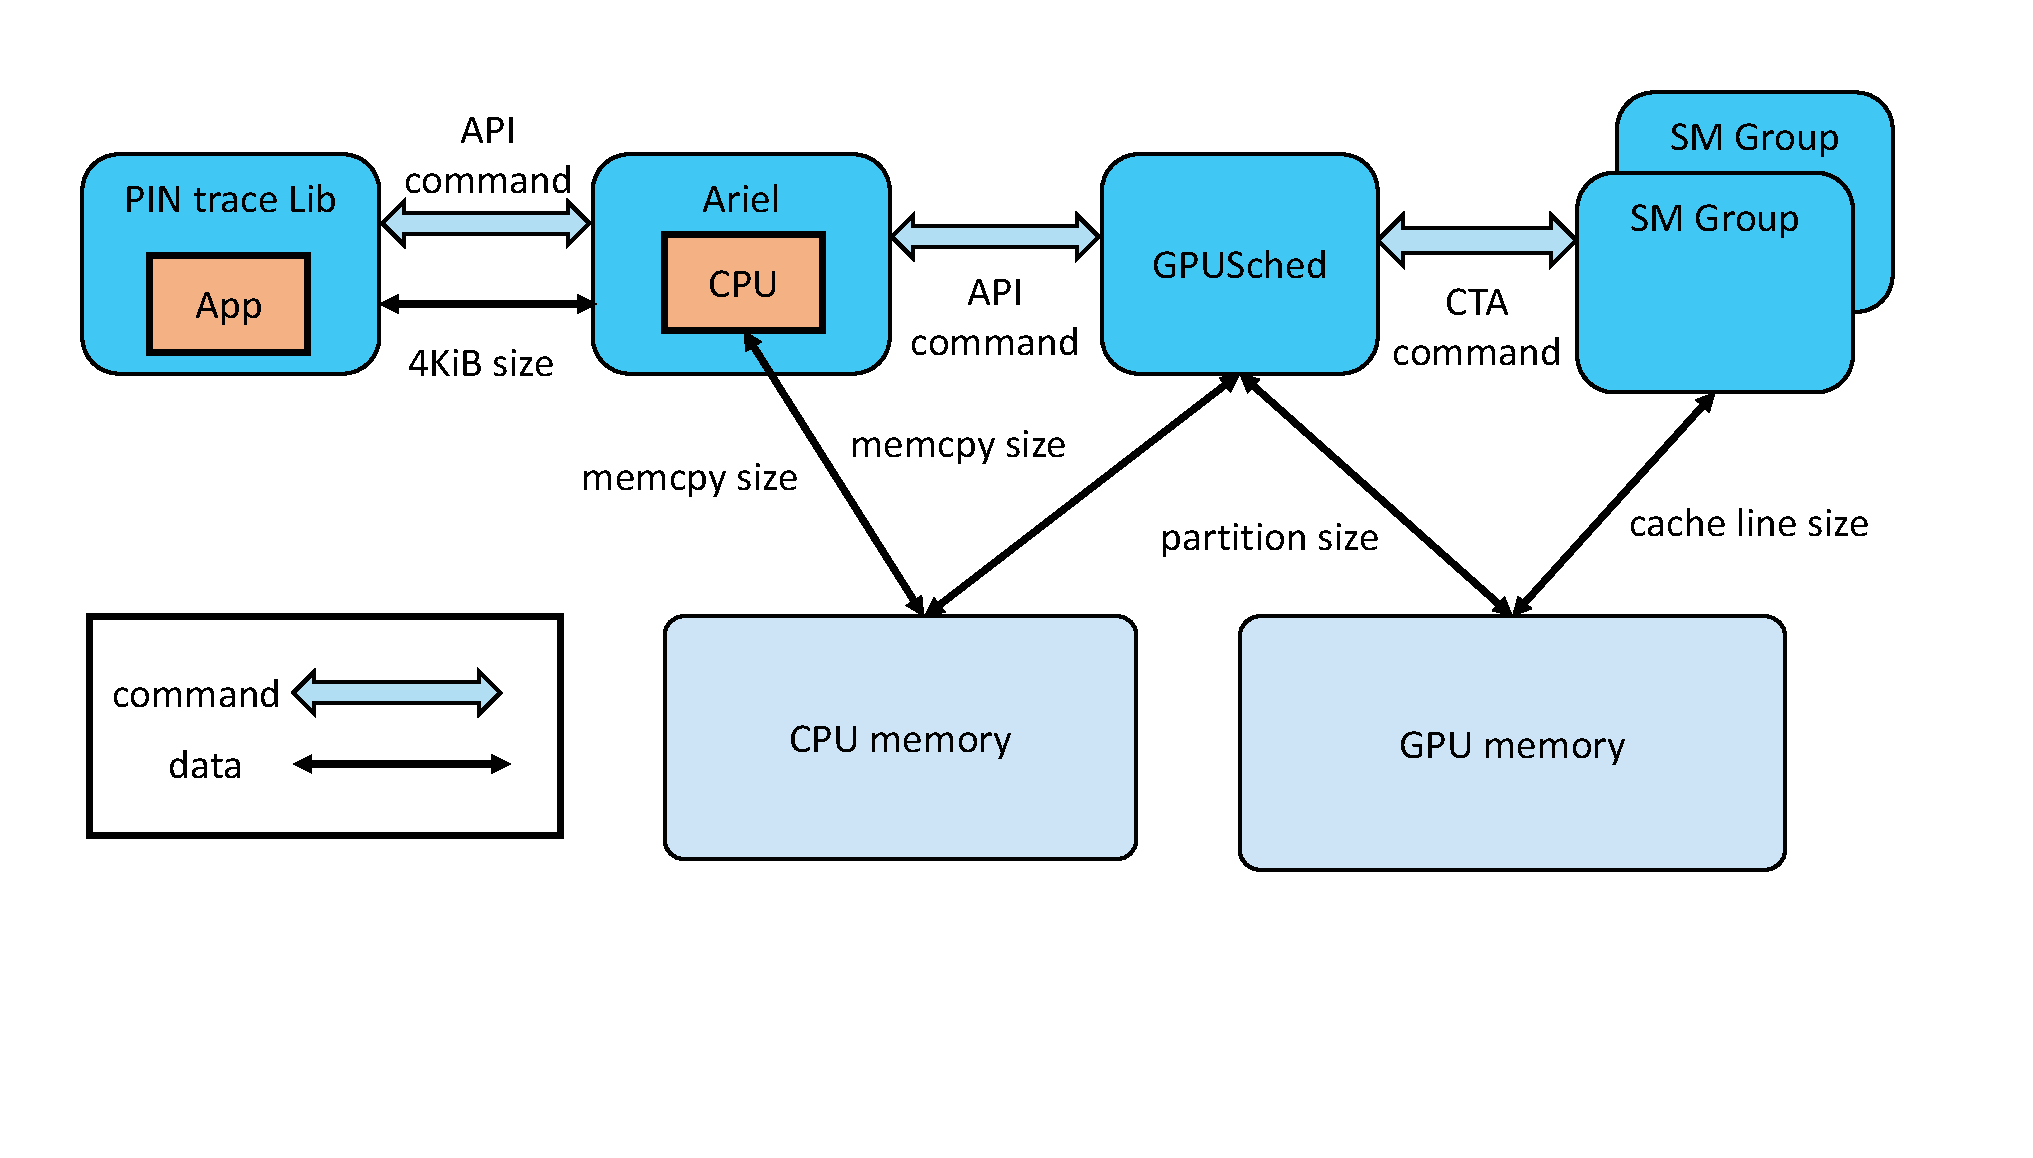
\includegraphics[width=.90\textwidth,keepaspectratio]{figures/transfer_flow.eps}
      \captionsetup{width=.75\textwidth}
      \caption{Data transfer flow for functional simulation}
      \label{fig:gpu_transfer_model}
   \end{figure}

Supporting the functional model of GPGPU-Sim also requires transferring values
from the CPU application to the GPU memory system. This is solved by leveraging
the link between CPU/GPU and memory hierarchy from SST, as shown in
\ref{fig:gpu_transfer_model}. Data are transferred from the application to Ariel through
inter-process communication tunnels. Ariel then communicates with the GPU scheduler through
the CPU memory. The GPU schduler then write the data to the GPU memory. When an SM
request a piece of data, the SM accesses the GPU memory for it.
The tunnels utilize 4KiB size as the granularity, while CPU and GPU components
employ larger size non-cacheable requests to access to CPU and GPU memories.

To model GPU performance, the memory system of the public GPGPU-Sim is
completely removed. Instead, all accesses to GPU memory are sent though SST
links to the MemHierarchy interface. As Figure \ref{fig:gpu_mem_model} shows, a
multi-level cache hierarchy is simulated with the shared L2 sliced between
different memory partitions, each with its own memory controller. Several
backend timing models have been configured and tested, including SimpleMem,
SimpleDRAM, TimingDRAM, and CramSim \cite{healy2017}; CramSim will be used to
model the HBM stacks in the more detailed performance models. We have created an
initial model for the GPU system similar to that found in an Nvidia Volta. The
configuration for the GPU, CramSim and Network components is shown in Listing
\ref{lst:sst_config}.


   \begin{figure}[!htb]
      \centering
      \setlength{\abovecaptionskip}{6pt plus 1pt minus 1pt}
      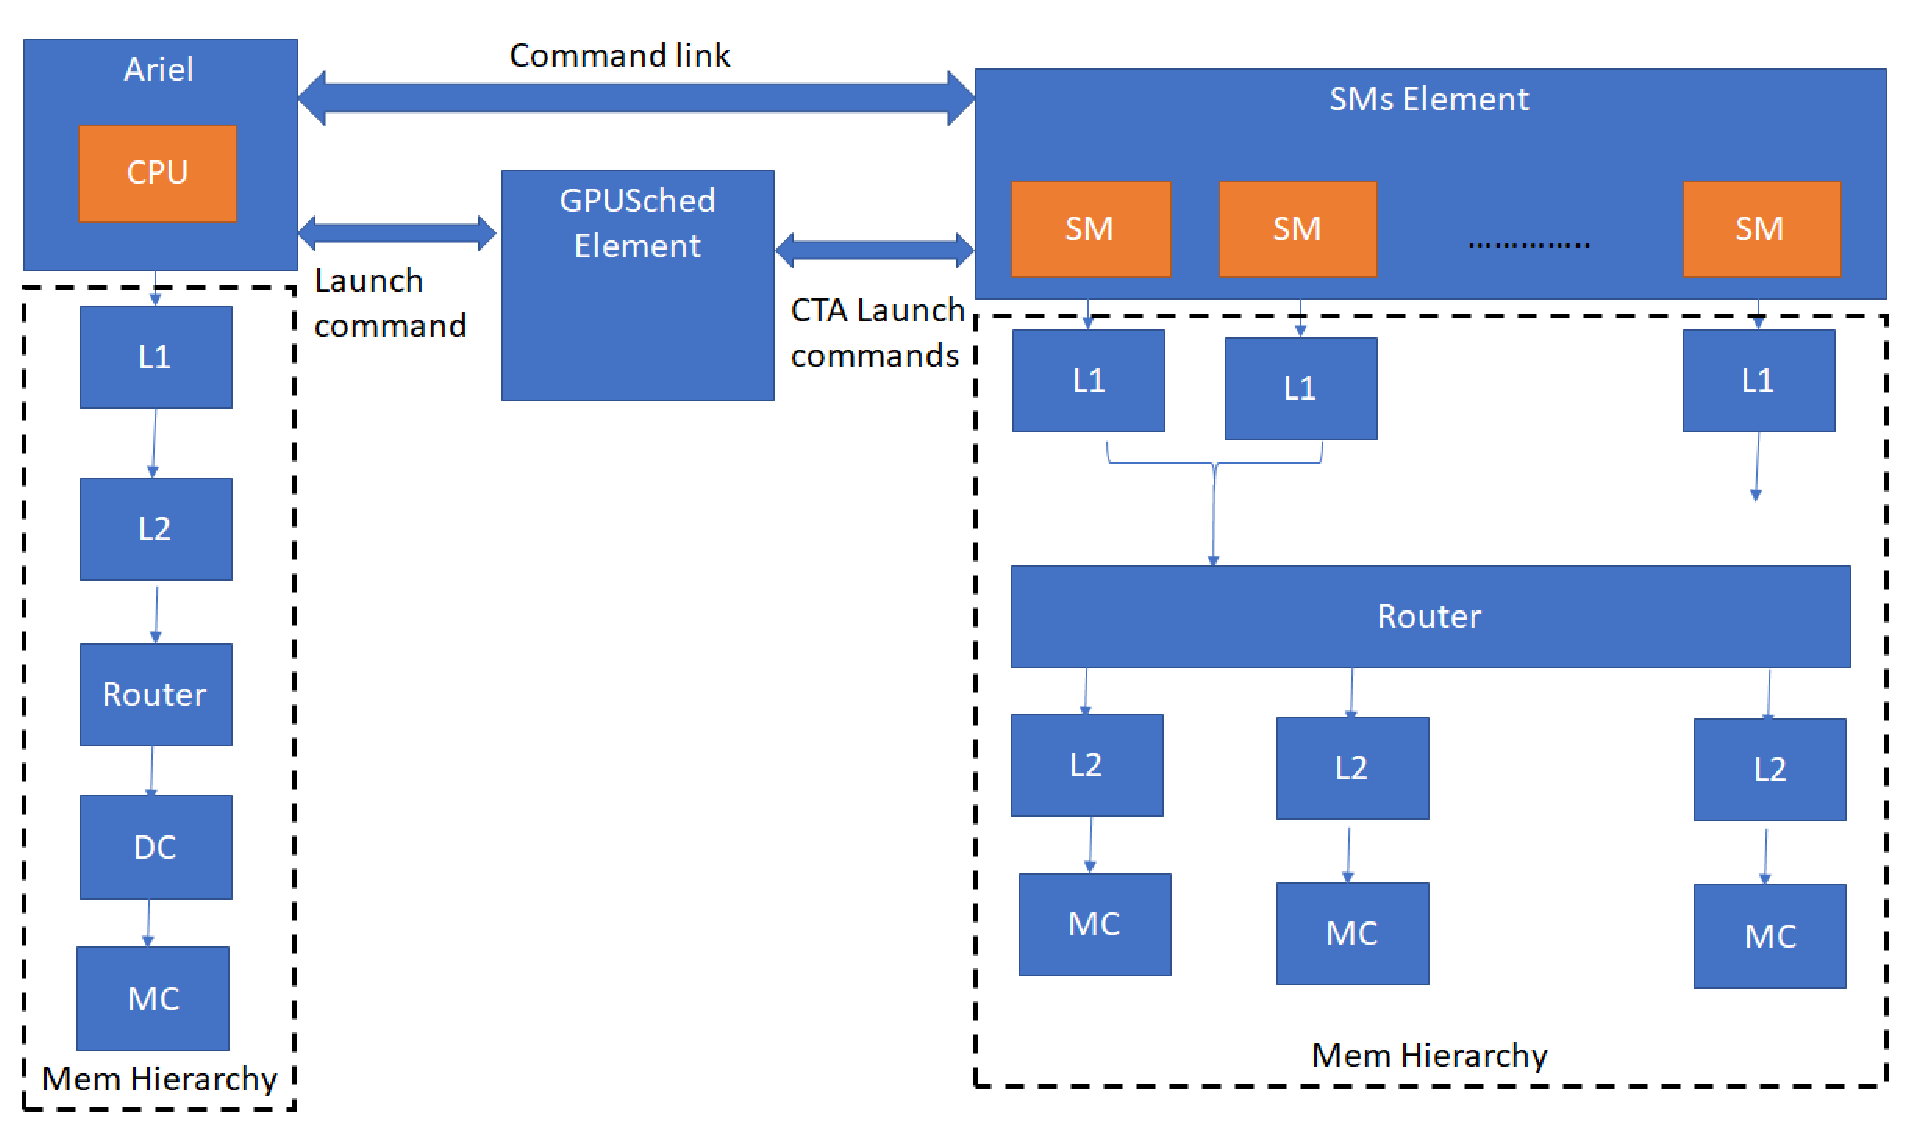
\includegraphics[width=.90\textwidth,keepaspectratio]{figures/3_1.eps}
      \captionsetup{width=.75\textwidth}
      \caption{Timing and memory model for SMs component}
      \label{fig:gpu_mem_model}
   \end{figure}


\clearpage
\lstdefinelanguage{mooCows}
{
  basicstyle={\small\ttfamily},
  columns=flexible,
  tag=[s]{[]},
  tagstyle=\color{dkgreen}\bfseries,
  usekeywordsintag=true
}[html]

\lstset{frame=tb,
  language=mooCows,
  aboveskip=3mm,
  belowskip=3mm,
  showstringspaces=false,
  columns=flexible,
  basicstyle={\small\ttfamily},
  numbers=none,
  numberstyle=\tiny\color{gray},
  breaklines=true,
  breakatwhitespace=true,
  tabsize=3
}

\lstinputlisting[caption=Sample SST-GPGPU Configuration, label=lst:sst_config]{figures/config}
\clearpage
